\begin{figure}[h] 
\centering 
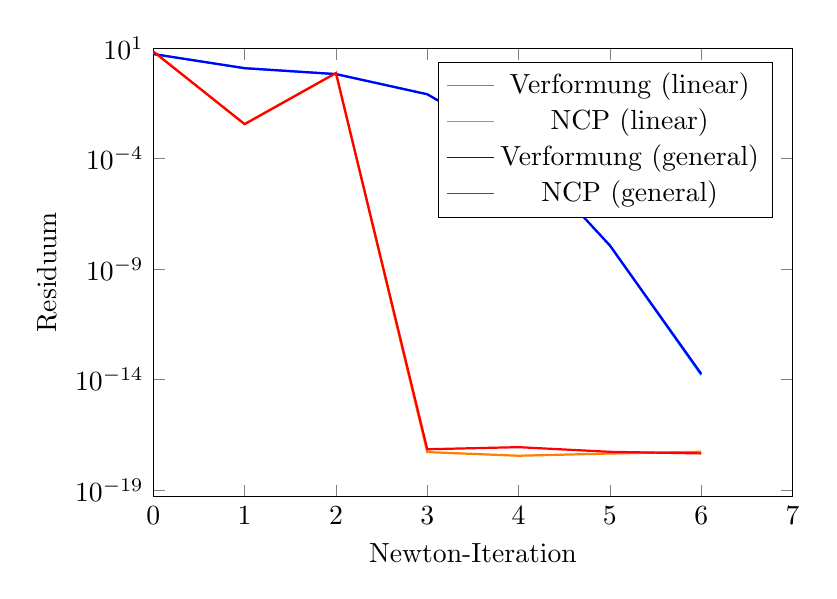
\begin{tikzpicture}[every plot/.append style={thick}] 
\begin{axis}[ 
label style={font=\normalsize}, 
xlabel={Newton-Iteration}, 
ylabel={Residuum}, 
xmin=0, xmax=7, 
ymode=log, 
ymin=0, ymax=10, 
width=0.8\textwidth, 
height=0.6\textwidth, 
legend pos=north east, 
legend style={cells={align=left}}, 
grid style=dashed, 
] 
\addplot[ 
color=cyan, 
] 
coordinates { 
(0, 5.42e+00)(1, 1.24e+00)(2, 6.70e-01)(3, 8.20e-02)(4, 3.45e-04)(5, 1.17e-08)(6, 1.61e-14)}; 
\addlegendentry{Verformung (linear)} 
\addplot[ 
color=orange, 
] 
coordinates { 
(0, 7.07e+00)(1, 3.65e-03)(2, 7.47e-01)(3, 5.23e-18)(4, 3.57e-18)(5, 4.50e-18)(6, 5.42e-18)}; 
\addlegendentry{NCP (linear)} 
\addplot[ 
color=blue, 
] 
coordinates { 
(0, 5.42e+00)(1, 1.24e+00)(2, 6.70e-01)(3, 8.20e-02)(4, 3.45e-04)(5, 1.17e-08)(6, 1.83e-14)}; 
\addlegendentry{Verformung (general)} 
\addplot[ 
color=red, 
] 
coordinates { 
(0, 7.07e+00)(1, 3.65e-03)(2, 7.47e-01)(3, 7.03e-18)(4, 8.73e-18)(5, 5.37e-18)(6, 4.55e-18)}; 
\addlegendentry{NCP (general)} 
\end{axis} 
\end{tikzpicture} 
\caption{Residuen des Stoffgesetzes 'Neo Hooke' mit Hinderniss 'Spitze' und 578 Freiheitsgraden für die Verschiebung.} 
\label{fiq:NeoHooke_Spitze_level3} 
\end{figure} 
